\subsubsection{16.04.15}
\begin{enumerate}
	
	\item The time of beginning and ending of the meeting: 1:00 - 2:00.
	
	\item Purposes of the meeting: 
	\begin{enumerate}
		
		\item Install plexiglass protection from the back.
		
		\item Connect the detail for directing balls vertically to the bucket.
		
        \item Change the construction of the MCB.
		
	\end{enumerate}

	\item Work that has been done:
	\begin{enumerate}
		
		\item We understood that the previous mechansm for capturing rolling goals can't be installed accurately, so we refused it. We decided to realise a project with servo fixed under the back carcase beam. We didn't do this project before as it unable to center goal, but now it centers by beams from wheel base, so it's ok.
		\begin{figure}[H]
			\begin{minipage}[h]{0.31\linewidth}
				\center{
\includegraphics[scale=0.13]{days/16.04.15/images/01}}
				\caption{New capture with goal}
			\end{minipage}
			\hfill
			\begin{minipage}[h]{0.31\linewidth}
				\center{
\includegraphics[scale=0.15]{days/16.04.15/images/02}}
				\caption{MCB opened}
			\end{minipage}
			\hfill
			\begin{minipage}[h]{0.31\linewidth}
				\center{
\includegraphics[scale=0.15]{days/16.04.15/images/03}}
				\caption{MCB closed}
			\end{minipage}
		\end{figure}
		
		\item Next, because of deinstalling the bottom plate (we installed new MCB instead if it), we needed to make new mount for the battery. We moved the battery closer to the lift, so it became easier to extract it.
		\begin{figure}[H]
			\begin{minipage}[h]{0.2\linewidth}
				\center  
			\end{minipage}
			\begin{minipage}[h]{0.6\linewidth}
				\center{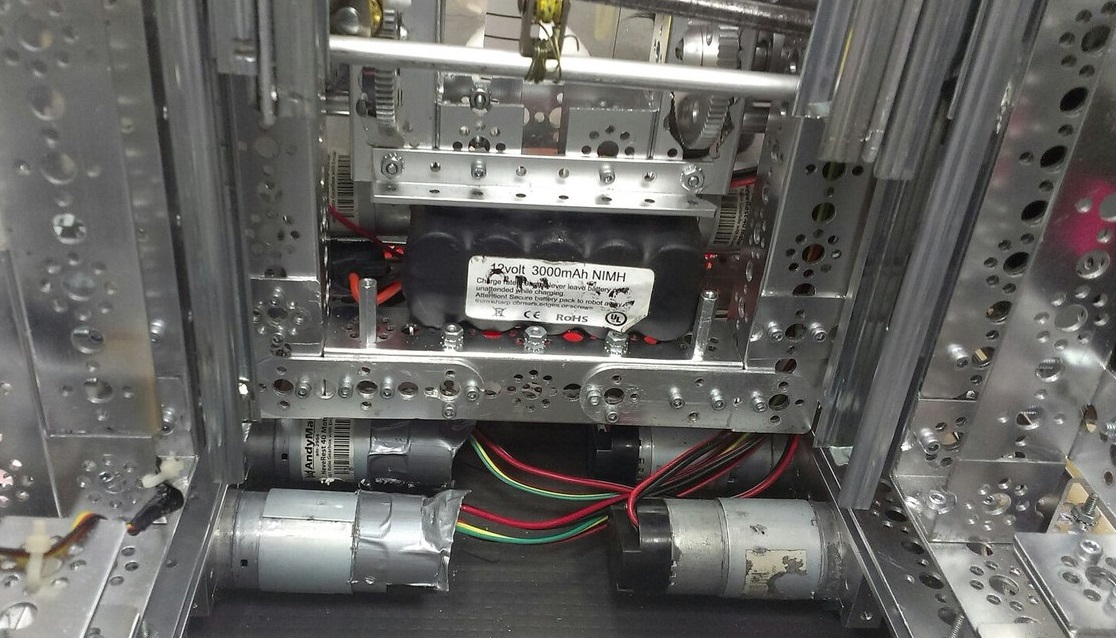
\includegraphics[scale=0.25]{days/16.04.15/images/04}}
				\caption{Battery in new mount}
			\end{minipage}
		\end{figure}
		
        \item We measured the sizes and cut out the back sheet of plexiglass. We left only 1,5 cm between the corner of of plexiglass and the ground (except hole for the rolling goal) to protect wheels from the small balls. Also we made holes for screws in the plexiglass.
        \begin{figure}[H]
        	\begin{minipage}[h]{0.2\linewidth}
        		\center  
        	\end{minipage}
        	\begin{minipage}[h]{0.6\linewidth}
        		\center{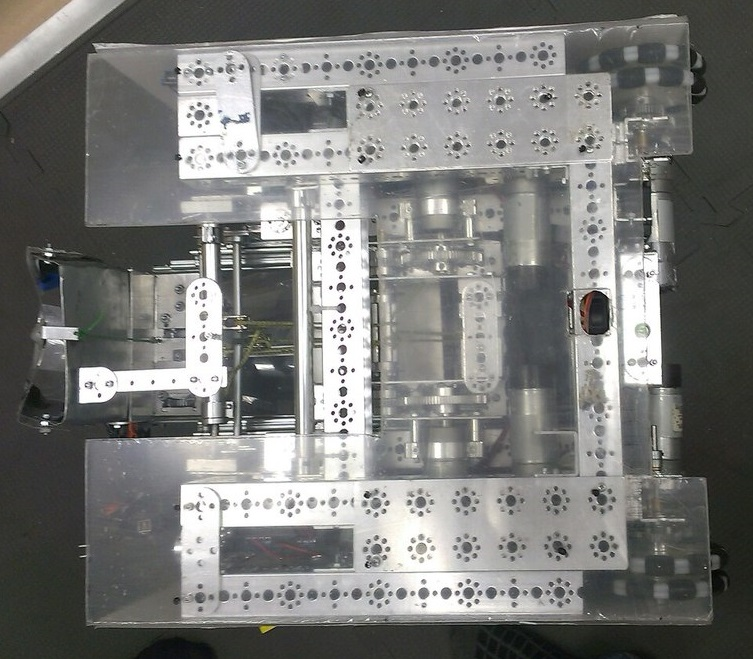
\includegraphics[scale=0.25]{days/16.04.15/images/05}}
        		\caption{The back sheet of the plexiglass}
        	\end{minipage}
        \end{figure}
        
        \item After we cut the plexiglass out, we started working on a sticker for it.
        
        \item We linked detail responsible for directing balls vertically with the bucket by the wire (as we detached it when we transported the robot by plane from Nederlands).
        \begin{figure}[H]
        	\begin{minipage}[h]{0.2\linewidth}
        		\center  
        	\end{minipage}
        	\begin{minipage}[h]{0.6\linewidth}
        		\center{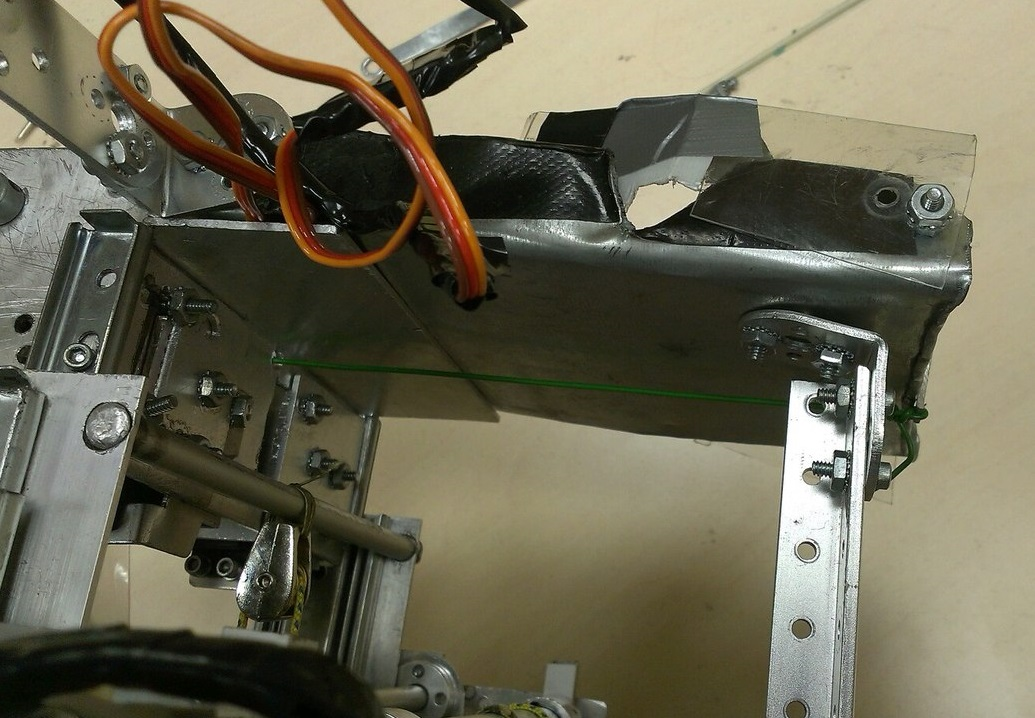
\includegraphics[scale=0.25]{days/16.04.15/images/06}}
        		\caption{The wire for opening the direct for balls.}
        	\end{minipage}
        \end{figure}
        
        \item In addition, we changed frameworks for autonomus programs as now we use 6 motors for moving and 2 for rising the lift.
        
        \item At the end of the day, during the training, robot lost 3 of it's wheels. at the following congregation we should fix wheels more reliable.

	\end{enumerate}
	
	\item Results:
	\begin{enumerate}
		
		\item The construction fo the MCB was changed to a more compact.
		
		\item Battery was moved to another place.
		
        \item We made the back sheet of plexiglass.
        
        \item Detail for directing balls vertically was connected to the bucket.
        
        \item Autonomus programs were corrected.
        
	\end{enumerate}
	
	\item Tasks for the next meetings:
	\begin{enumerate}
		
		\item Fix wheels more reliable.
		
		\item Create autonomus programs.
			
	\end{enumerate}
\end{enumerate}
\fillpage
